\section{Eksisterende Systemer}
Dette afsnit detaljerer eksisterende systemer som allerede implementerer mange af de ting der er tiltænkt dette projekt eller har lignende funktionalitet, såsom fitness applikationer. 
Systemerne der vil blive forklaret er Ginger.io, Apple Health, Google Fit, Microsoft Health og Healthvault.

\subsection{Ginger.io}
Ginger.io er en applikation til iPhone og Android, beregnet til at assistere patienter med diverse psykiske lidelser.\cite{ginger_dot_io}\cite{gingerio_mit}\cite{gingerio_dailymail}


Applikationen er lavet til at assistere i behandlingen for følgende lidelser: depression, angst, bipolær affektiv lidelse og skizofreni.

Efter at applikationen er installeret, vil den indsamle data, denne data kan så bruges til at sige noget om mobil-brugerens sindsmæssige tilstand.
Der bliver overordnet set indsamlet to typer data; aktiv og passiv.
Aktiv data er forespørgsler fra applikationen, hvor mobil-brugeren selv skal svare.
Passiv data vil blive indsamlet i baggrunden, og består af interaktions- og lokations-data, hvor interaktions-data er mobil-brugerens opkald- og SMS-vaner og lokations-data er opfanget via GPS og accelerometer, for at sige noget om hvor og hvordan mobil-brugeren bevæger og opholder sig.

For at komme i gang med applikationen, skal brugeren indtaste relevant information, såsom diagnoser, behandlingsforløb og behandler.
Ud fra disse informationer vil applikationen tilpasse forespørgslerne brugt til indsamling af aktive data.
Derudover vil passiv data der indsamles i de første dage bruges til at angive brugerens normal-tilstand.
Herefter vil brugeren modtage notifikationer om ændring i social eller fysisk aktivitet, og i værste tilfælde vil behandler eller anden angivet kontaktperson blive notificeret.

Brugere af Ginger.io skal være forbundet gennem en behandler, og denne behandler vil til enhver tid have adgang til alle brugerens informationer.
Den overordnede idé er at Ginger.io skal assistere behandlingsprocessen, ved at give en indikator på brugerens tilstand mellem klinikbesøg (se \cref{eksisterende_systemer:ginger_io_graf}).

\begin{figure}[h]
\centering
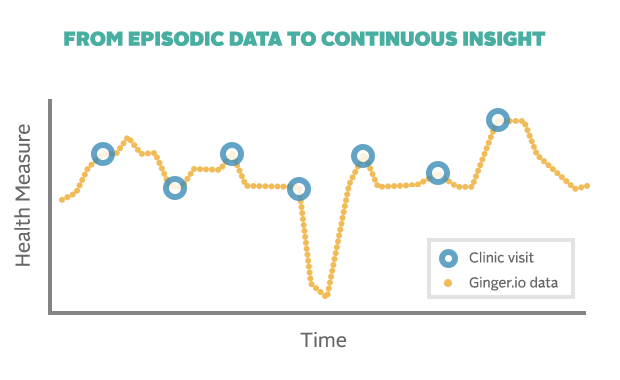
\includegraphics[width=.75\textwidth]{ginger_io_graph}
\caption{Figur fra https://ginger.io/for-providers/}
\label{eksisterende_systemer:ginger_io_graf}
\end{figure}

\subsubsection{Problemer}
Som det ser ud nu, er Ginger.io kun tilgængeligt i USA, og kun ved tilmeldte behandlere.
Derudover fungerer interaktions-data-indsamlingen kun på Android, hvilket betyder at iPhone applikationen kun indsamler data omkring lokation, samt aktiv data.

\subsection{Fitness Trackere}
Der findes adskillige applikationer og større systemer til at styre ens fysiske aktivitet og velvære.
Heriblandt;
\begin{itemize}
\item Apple Health\cite{apple_health}
\item Google Fit\cite{google_fit}\cite{google_fit_api}
\item Microsoft Health\cite{ms_health} og HealthVault\cite{ms_health_vault}\cite{ms_health_vault_api}
\end{itemize}

Ens for disse fitness trackere, i modsætning til enkelte applikationer, er at de samler informationer fra et væld af forbundne enheder og applikationer.
Ydermere kan de indstilles til bestemte mål, og derved løbende fortælle om hvordan det går med at opnå disse mål.

\subsubsection{Apple Health}
Med Apple Health er det muligt at indsamle information fra andre applikationer (fx. måltider eller hjertefrekvens), for at samle al data ét sted på sin mobil, eller synce det med en iCloud konto.
Derudover er det muligt for andre applikationer at få adgang til Apple Health's data, ved at give tilladelse til forskellige kategorier af data.
Skærmbilleder af henholdsvis den oversigt Apple Health kan give, samt de kategorier der indsamles i, kan ses på \cref{eksisterende_systemer:apple_health_ss}.

\begin{figure}
\centering
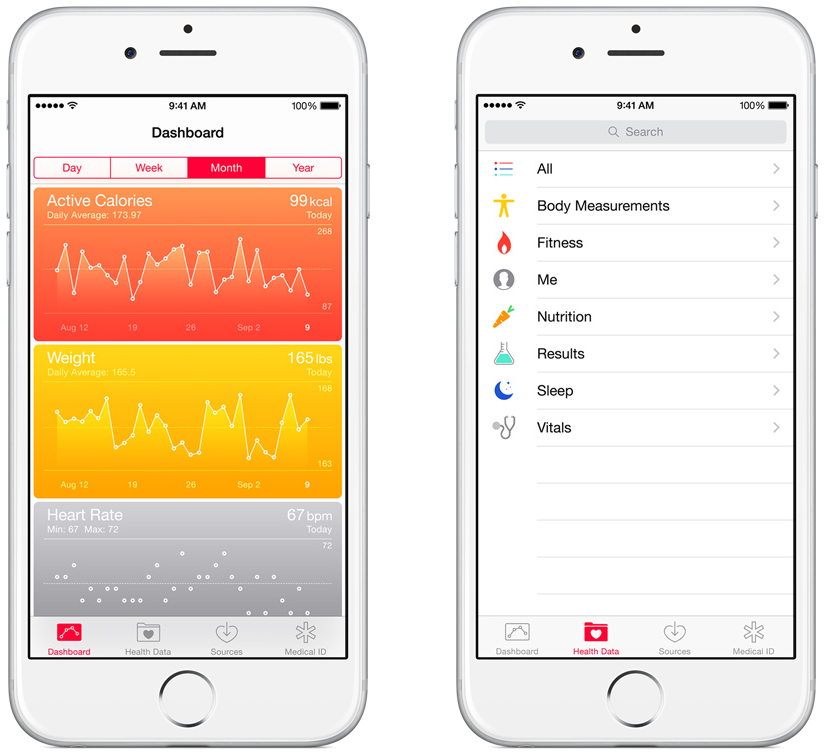
\includegraphics[width=.75\textwidth]{apple_health_ss}
\caption{Skærmbilleder af Apple Health fra \url{https://www.apple.com/ios/whats-new/health/}}
\label{eksisterende_systemer:apple_health_ss}
\end{figure}

\subsubsection{Google Fit}
Ligesom Apple Health, kan Google Fit samle data fra andre applikationer.
Derudover kan Google Fit også indsamle data fra andre kilder, såsom wearables.
Derefter er det muligt at få oversigt over ens aktiviteter og fysiske tilstand, via Googles egen side eller applikation.
Det er også muligt at lave sine egne applikationer, til både indsamling og visualisering, via Google Fit API (Android SDK eller REST web service).

Uden eksterne wearables eller applikationer, indsamles der kun bevægelses-data fra fx. GPS, hvor Google Fit applikationen selv estimerer om man går, løber eller cykler.
For andet aktivitet skal man manuelt indtaste (fx. roning eller yoga) sammen med varigheden.

Google Fit består af 4 komponenter:

\begin{description}
\item[Fitness store] er hvor de indsamlede data er gemt.
\item[Sensor framework] indeholder alt der skal bruges for at indsamle og repræsentere data, gennem repræsentationerne: \textit{Data Sources, Data Types, Data Points, Datasets, Sessions}.
\item[Permissions and User Controls] styrer adgang til de 3 data-kategorier: \textit{activity, location, body}.
Der gives læse eller læse+skrive rettigheder til én eller flere kategorier.
\item[Google Fit APIs] dækker over Android SDK og REST web service.
\end{description}

\subsubsection{Microsoft Health og HealthVault}
Microsoft Health er det overordnede system, som kan ses på \cref{eksisterende_systemer:ms_health_fig}.
HealthVault er hvor de indsamlede data er samlet og gjort tilgængelig for andre applikationer, via en web service.
Applikationer der vil gøre brug af HealthVault skal anmode om specifikke rettigheder (såsom til allergi-informationer eller mad-indtag).
I skrivende stund er der kun SDK til .NET framework.

Ud over at indsamle data fra smart devices og wearables, kan man i HealthVault også uploade dokumenter såsom røntgenbilleder.
Idéen er at man skal samle alle helbreds oplysninger ét sted, ikke kun dem vedrørende fitness.

Der er 4 vigtige koncepter i HealthVault:
\begin{description}
\item[Record] er medicin og fitness information for en enkelt person.
\item[Person] er et individ, som har fuld adgang til sin egen \textbf{Record}, med mulighed for at få adgang til andre personers records.
\item[Thing] er noget bestemt data gemt i en \textbf{Record}.
\item[Thing type] er typen for en \textbf{Thing}, hvilket beskriver hvad det er for en måling (såsom vægt eller blodtryk).
\end{description}

\begin{figure}
\centering
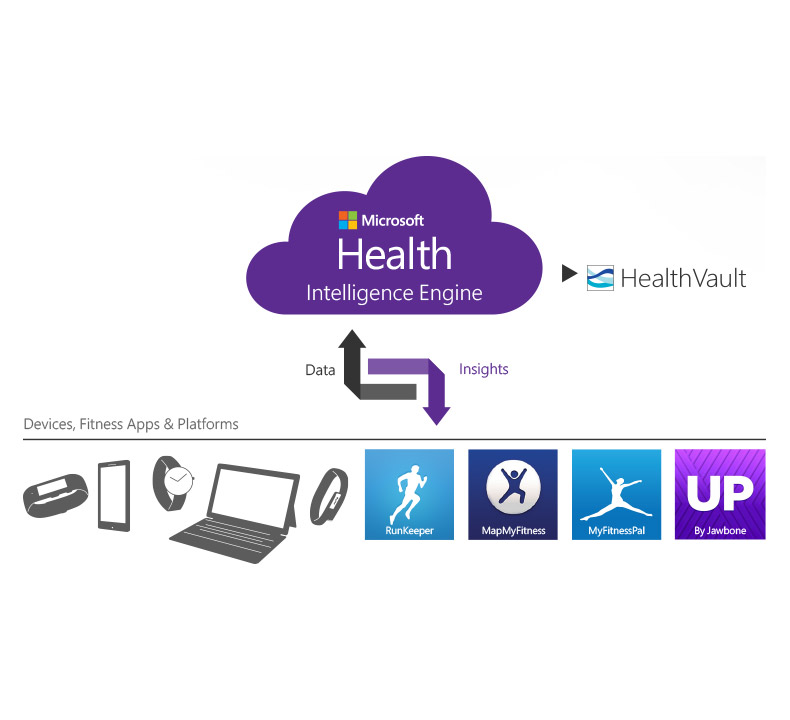
\includegraphics[width=\textwidth]{ms_health}
\caption{Microsoft Health fra \url{http://www.microsoft.com/microsoft-health/en-us}}
\label{eksisterende_systemer:ms_health_fig}
\end{figure}

\subsubsection{Problemer}

\paragraph{Apple Health}
Apple Health er naturligvis lukket til iOS.
Som det er nu, er det ikke muligt at dele helbredsoplysninger direkte med andre personer.
Som det er nu skal der laves eksterne applikationer til indsamling af data, Apple Health kan ikke selv tilslutte sig wearables for at indsamle data.
\ivan{Bør checkes, hvad med Watch?}

\paragraph{Google Fit}
Ifølge Google Fit Terms and Conditions er det ikke tilladt at bruge Google Fit til andet end fitness-formål, fx. at gemme lægelige eller biometriske data.\footnote{''Do not use Google Fit APIs for non-fitness purposes, such as storing medical or biometric data, selling data, or using data for advertising.''}
Lægelige data dækker over lægefaglige data, såsom diagnoser og sygdomsforløb.
Biometrisk data dækker over data som kan identificere en person, såsom iris-skan eller stemmemønster.

\paragraph{MS Health og HealthVault}
Ved brug af MS Health er det kun muligt at hente data ned, efter det er i skyen.
Det vil sige at det ikke er muligt at få fat i rå data, som ved Google Fit.
På nuværende tidspunkt er der ingen SDK'er til MS Health, det er kun muligt at få adgang til data via web service'en.
